\documentclass{article}
\usepackage[utf8]{inputenc}
\usepackage[swedish]{babel}
\usepackage{authblk}
\usepackage{biblatex}
\addbibresource{sources.bib}
\usepackage{graphicx}

\title{ProjektRapport 14}
\author{Alamin Alreda \and Sebastian Danckwardt \and Isac Holm \and Zaid Haj Ibrahim   \and Edvin Svahn}
\date{September 2022}

\begin{document}

\maketitle

\section*{Ordlista}
Lista över beteckningar som används i denna rapport.
\begin{description}
    \item[USART] Universal Synchronous/Asynchronous Reciever/Transmitter är kopplingen mellan kortet och terminalen
    \item[CAN] Controller Area Network är ett protokoll som tillåter korten att kommunicera med varandra utan hjälp av en dator. Detta görs med två bussar som sitter på korten
    \item[Buss] En buss är en kommunikationsport som kan användas för att utbyta information
    \item[MD-kort]
    \item[GPIO] General Purpose Input Output är en anslutning på korten dit man kan koppla olika logiska enheter som antingen tar emot eller skickar data.
    
\end{description}
 
\section{Introduktion}
Det här kapitlet svarar på frågor som varför projektet genomförs,
vad som förväntas uppnås av projektet samt hur gruppen arbetar för att uppnå ett resultat.
\subsection{Syfte}
Varför?
\\
Bara under 2021 har 72 884 fall av inbrottsstöld anmälts\cite{BRa}. 
Cirka 20\% svarar att de inte har ett hemlarm för att det helt enkelt är för dyrt\cite{MoFor}.
Genom att skapa ett system med ett billigt md407-kort kan man sänka kostnaderna för denna produkt och bekämpa brott i alla områden i Sverige. 
Projektet syftar till att skapa ett lättanvändligt och billigt larmsystem för att skydda mot stöld. 
Detta då endast 29\% av Sveriges befolkning idag använder ett larmsystem\cite{SSF}.
\subsection{Mål}
Vad?
\\
Målet med projektet är att konstruera ett larm/lås-system med två olika larmenheter: 
den ena ska kunna upptäcka i fall en dörr står öppen och den andra ska detektera rörelse och vibrationer. 
En central styrenhet ska utgöra den del av larmsystemet som har i uppgift att kommunicera med de fristående larmenheterna. 
Detta ska möjliggöra centraliserad kontroll och kalibrering av flera periferienheter i ett större larmsystem. 
Ytterligare en periferienhet ska simulera ett defekt larm i syfte för testning.
\\\\
När den centrala styrenheten startar ska en förfrågan skickas till de anslutna periferienheterna därpå de svarar med dess typ och konfiguration för att sedan tilldelas ett unikt ID. De olika larmenheterna ska inledningsvis larma lokalt med en röd lysdiod, om specifika krav nås meddelas den centrala styrenheten. Dörrlarmet larmar till centralenheten efter en bestämd tid medans rörelsesensorn måste upptäcka rörelse på ett visst avstånd. Det ska även vara möjligt att låsa/låsa upp dörren samt inaktivera dörrlarmet genom att mata in en fyrsiffrig kod på en keypad.


\subsection{Arbetsmetod}

\subsubsection{Planering}
Projektet inleddes med att projektgruppen fastställde ett kontrakt om hur möten, kommunikation och annat skulle gå till. Detta gjorde det lättare att börja arbeta genast under mötena, eftersom protokollet för mötet redan var känt i förväg och alla visste vad de kunde förvänta sig. Som en viktig sak var det bland annat viktigt att kommunicera problem med de andra i gruppen så att ingen fastnar.

Vi definierade de mål som vi ville uppnå och deadlines för varje mål. Vi ville också ha en tydlig struktur för projektet och ha en tydlig överblick över hur projektet utvecklas. Därför använde vi ett Gantt-diagram med tydliga milstolpar för vår projektplanering. Gantt-diagrammet gav oss en tydlig överblick av projektet och gjorde det lätt för oss att se vad som gjordes och vad som fortfarande behövde göras. De båda hjälpte oss också att fastställa och hålla reda på deadlines. Dessutom hade vi även en discord-kanal där vi snabbt kunde kommunicera med varandra och arbeta på ett smidigt sätt tillsammans även på distans.

Det var viktigt att ha möten flera gånger i veckan för att föra projektet framåt och se till att ingen fastnade. Varje möte inleddes med att skriva ner vad varje individ skulle arbeta med under mötet, vad de gjorde under föregående möte och sedan om de behöver hjälp med det de gör under dagen.  I slutet av varje möte tittade vi på vad vi hade gjort och vad som fortfarande behövde göras för att se till att vi var på rätt spår med vårt projekt.

\subsubsection{Process}
När gruppen började skriva kod för projektet delades den upp i två undergrupper som var och en arbetade självständigt med separata delar av projektet. Undergrupperna arbetade parallellt med varandra på distansmätaren och vibrationssensorn från början tills de var klara och sedan gick vidare till nästa del av projektet.

Vi genomförde också rigorösa tester när en funktion var färdig eller behövde testas genom att följa en testplan som hela gruppen enades om. Detta säkerställde att den nya koden integrerades väl med den befintliga koden och att den fungerade som det var tänkt. Vi använde också ett versionskontrollsystem för att hålla reda på ändringar i koden och för att enkelt kunna återgå till en äldre version om något gick fel.

Projektgruppen hade också regelbundna möten med projektledaren, där vi gick igenom vad vi hade gjort under föregående vecka, vad vi arbetade med under den aktuella veckan och om vi hade några problem. Detta hjälpte oss att hålla projektet på rätt spår och se till att vi gjorde goda framsteg.


\section{Teknisk beskrivning}
I det här kapitlet redogörs projektets tekniska bedrifter. 
I den tekniska bakgrunden beskrivs varför systemet är uppbyggt av de delar som det är.
Därefter ger Systemöversikten en övergripande förståelse för hur systemet är uppbyggt och sist men inte minst förklarar Delsystem hur delarna är uppbyggda.


\subsection{Teknisk bakgrund}
Vad är utgångspunkten för konstruktionsarbetet?

\subsection{Systemöversikt}
Hur ser det konstruerade systemet ut på en övergripande nivå?

\newpage

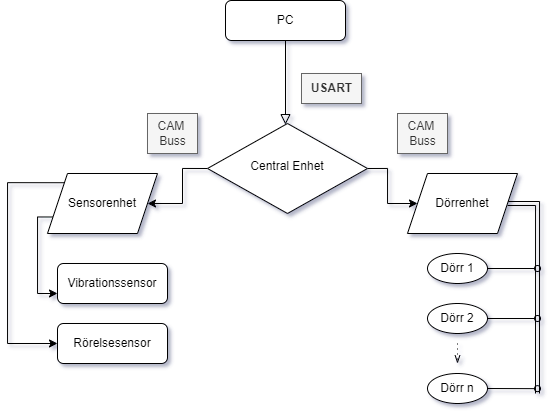
\includegraphics[scale=0.6]{Projektrapport/diagram.png}
\caption {Blockschema av larmsystemet}
\label{fig:drawing}


Systemet består i stort av tre delar - en centralenhet och två periferienheter. Utöver dessa enheterna innehåller systemet övriga delenheter som bidrar till funktionalitet av systemet i sin helhet. Ett md407-kort används som en ARM-processor för att koppla ihop olika instrument beroende på deras funktion och uppgifter (figure 1). Kommunikation mellan samtliga md-kort sker via CAN-buss, medan kommuniaktion mellan centralenheten och pc sker över USART. \\


Periferienhet 1 ska vara ansluten till en kopplingsplatta, på plattan ska det finnas lampor och en dörr-strömbrytare. Lamporna kommer lysa rött efter att dörren har varit öppen en viss tid eller grönt om inget larm har gått. Dörr-strömbrytarna kommer att simulera dörröppning eller dörrstängning. \\

Periferienhet 2 ska vara kopplad till en avståndsmätare (HC-SR04) och en vibrationssensor (SW-18010P). Avståndmätaren kommer att skicka en signal om avståndet har ändrats. På samma sätt kommer vibrationssensorn skicka en signal om den har känt av några vibrationer. \\


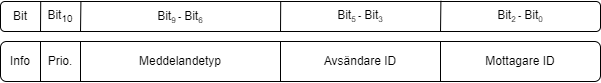
\includegraphics[scale=0.5]{Projektrapport/protokoll.png}

\subsection{Delsystem}
Hur ser det delar som ingår i systemet ut?
\subsubsection{Centalenhet}
Centralenheten kommunicerar ständigt med dörrenheten och sensorenheten över en CAN buss, denna komunikation kommer att omfatta ACK-, larm-, och konfiguration meddelanden. Dessutom ska centralenheten hantera all kommunikation mellan användaren och systemet genom USART. För att användaren ska få tillgång till systemet ska hen skriva in rätt lösenord. Därefter ska användaren kunna, för varje dörr, slå på eller av centrla larmet, ändra tröskelvärdet,låsa eller låsa upp dörren. Utöver det ska användaren också kunna ändra tröskelvärdet för avståndsmätaren.



\subsubsection{Dörrenhet}

Dörrenheten kommer att vara kopplad till flera dörrar, där varje dörr kommer att vara kopplad till en grönlapma, en rödlampa och ett lås.Utöver det kommer varje dörr att ha sitt eget tröskelvärde som bestämmer när larmet ska gå av. När tiden har gått ett tröskelvärde kommer det lokala larmet att gå av och det kan man se genom att den röda lampan lyser. Efter två tröskelvärden kommer dörrenheten att skicka till centralenheten för att påställa störenheten. Om dörren är stängd ska den gröna lampan lysa medan det lokala och centrla larmet ska vara avstängda. 

\subsubsection{Sensorenhet}

Sensorenheten kommer att vara kopplad till två sensorer; avståndsmätare och vibrationsensor (HC-SR04 respektive SW-18010P).Avståndsmätaren kommer att läsa av avståndet till ett objekt genom att skicka ultraljudssignaler och vänta på att få tillbaka ett eko. Mättningen av avståndet kommer att ske genom att räkna skillanden i mikrosekunder mellan ultraljudssignaler och deras eko, därefter divideras tiden med 58 för att få avståndet i centimeter. Avståndet kommer att mättas kontinuerligt i intervaller av 60 millisekunder, om avståndet överstiger eller blir mindre än tröskelvärdet kommer det centrala larmet att gå av.\\
\\
Å andra handen kommer också vibrationsensor att känna av vibrationer, ifall den känner av någon vibration kommer den att den skicka till centralenheten för att slå på störenhetn.



\section{Resultat}
Detta avsnitt redovisar resultatet av genomförd verifiering av systemet; dels för delarna, dels för komplett system. 
Detta avsnitt redovisar även resultatet av det slutliga fysiska testet när hela systemet körs i skarpt läge. 
Ni ska främst redovisa resultat i form av funktionalitet, men ta också upp prestanda aspekter om dessa är viktiga.  

\section{Slutsatser}


\newpage
\section{Källförteckning}
\printbibliography[heading=none]

\end{document}
